\chapter{SLAM эксперименты}

Для проверки возможности использования SLAM методов совместно с методами построения и восстановления карты местности в реальном, было решено имитировать поток данный с БПЛА с помощью внешней usb веб-камеры.

\section{Настройка и калибровка камеры}

Для работы с usb веб-камерой через ROS, требуется использовать пакет \textbf{cv-camera} который предоставляет узел, взаимодействующий с камерой и принимающей от неё поток видео.

Как и во всех задачах компьютерного зрения, перед началом работы, требуется откалибровать камеру - т.е. получить её внутренние и внешние параметры. С помощью калибровки получаются такие параметры, как: фокусное расстояние, угол наклона, и принципиальная точка (соответствует центру фотографии) - которые образуют так называемую матрицу камеры и коэффициенты дисторсии (искажения).

\begin{figure}[h]
    \centering
    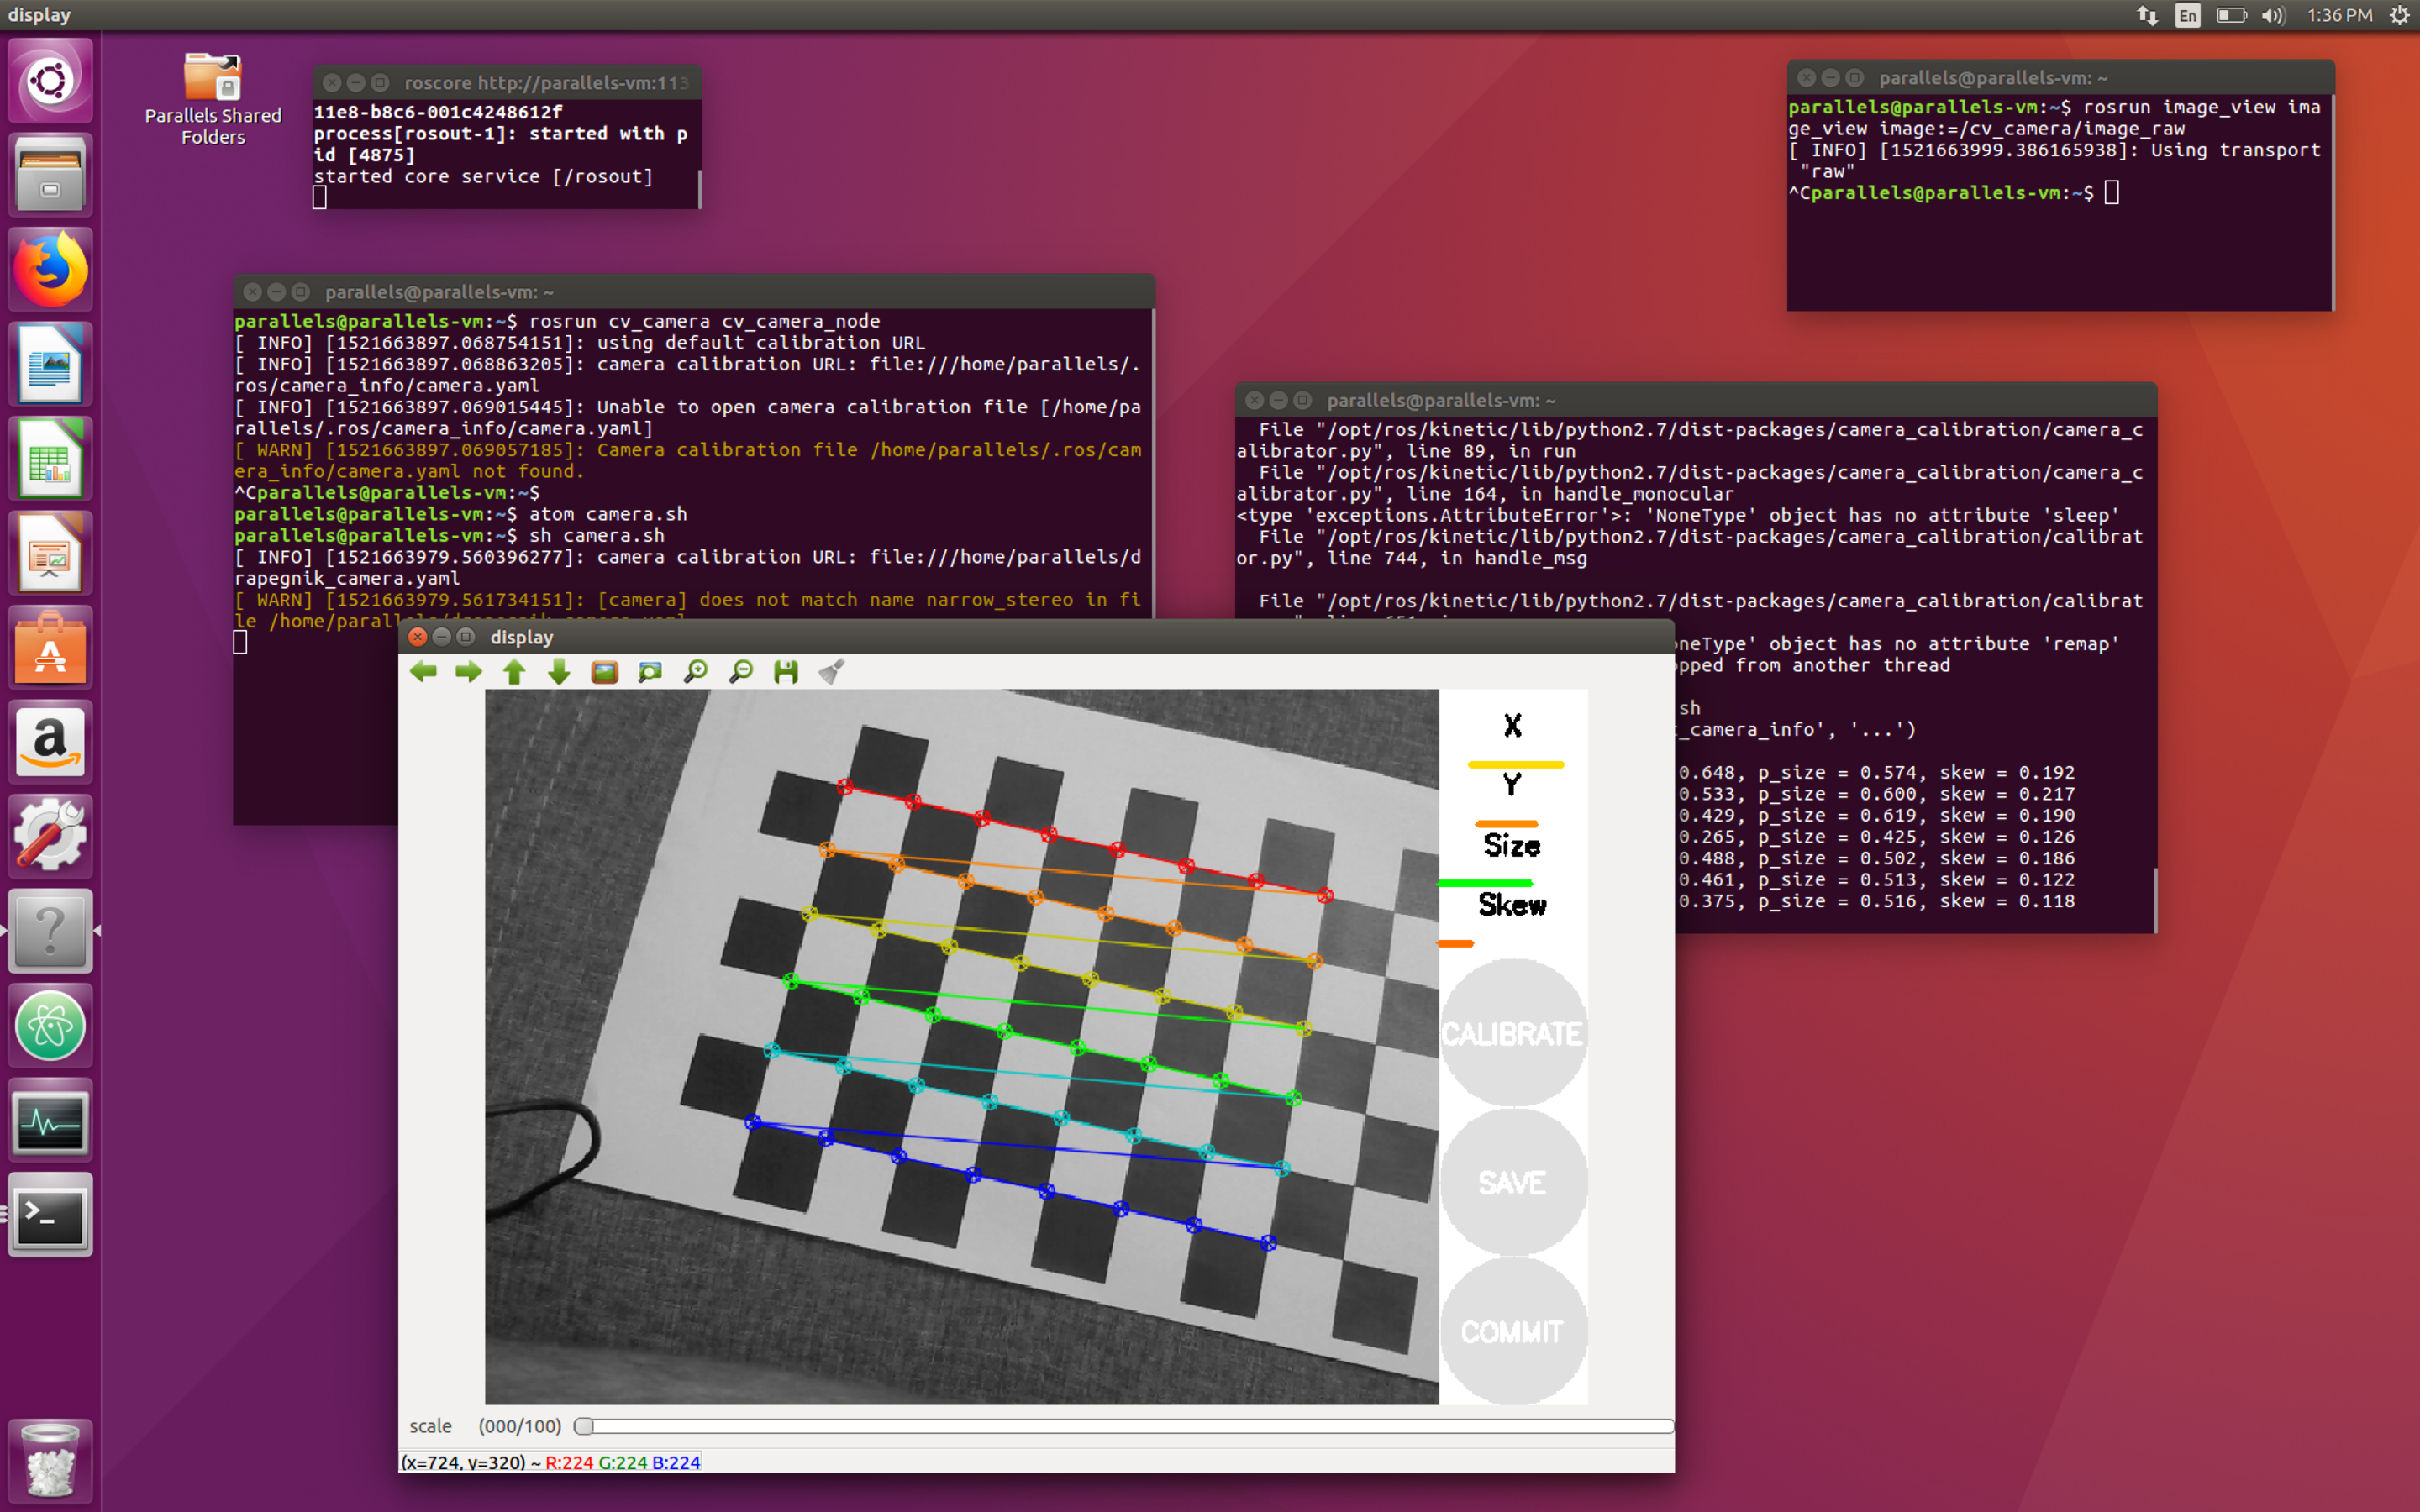
\includegraphics[width=0.9\textwidth]{images/chess.png}
    \caption{Калибровка камеры с помощью шахматной доски}
    \label{fig:chess}
\end{figure}

Обычная процедура калибровки представляет из себя следующее:

\begin{enumerate}
    \item выбор предмета с известной геометрией, обычно используется изображение шахматной доски;
    \item подготовка 30 или более изображений выбранного предмета с разных ракурсов и расстояний;
    \item определение ключевых точек на полученных фотографиях;
    \item определение коэффициентов дисторсии через минимизацию ошибки.
    \item нахождение остальных параметров через уравнения, полученные путем сопоставления изображений.
\end{enumerate}
 
Полученные параметры камеры экспортируются в файл и используются для конфигурации SLAM алгоритмов.

\section{Связывание через ROS}

Для того, чтобы использовать всё вышеописанное вместе, потребуется следующее: один узел отвечает за веб-камеру - принимает от неё видео поток и публикует его в специальный канал - \textbf{/cv\_camera/image\_raw}. SLAM запускается как отдельный узел и подписывается на этот канал, получая данные выполняет задачу позиционирования и построения разряжённой карты точек. Полученные результаты экспортируются и далее могут быть использованы для уточнения результатов и ускорения времени работы алгоритма построения плотной карты местности.

\begin{figure}[h]
    \centering
    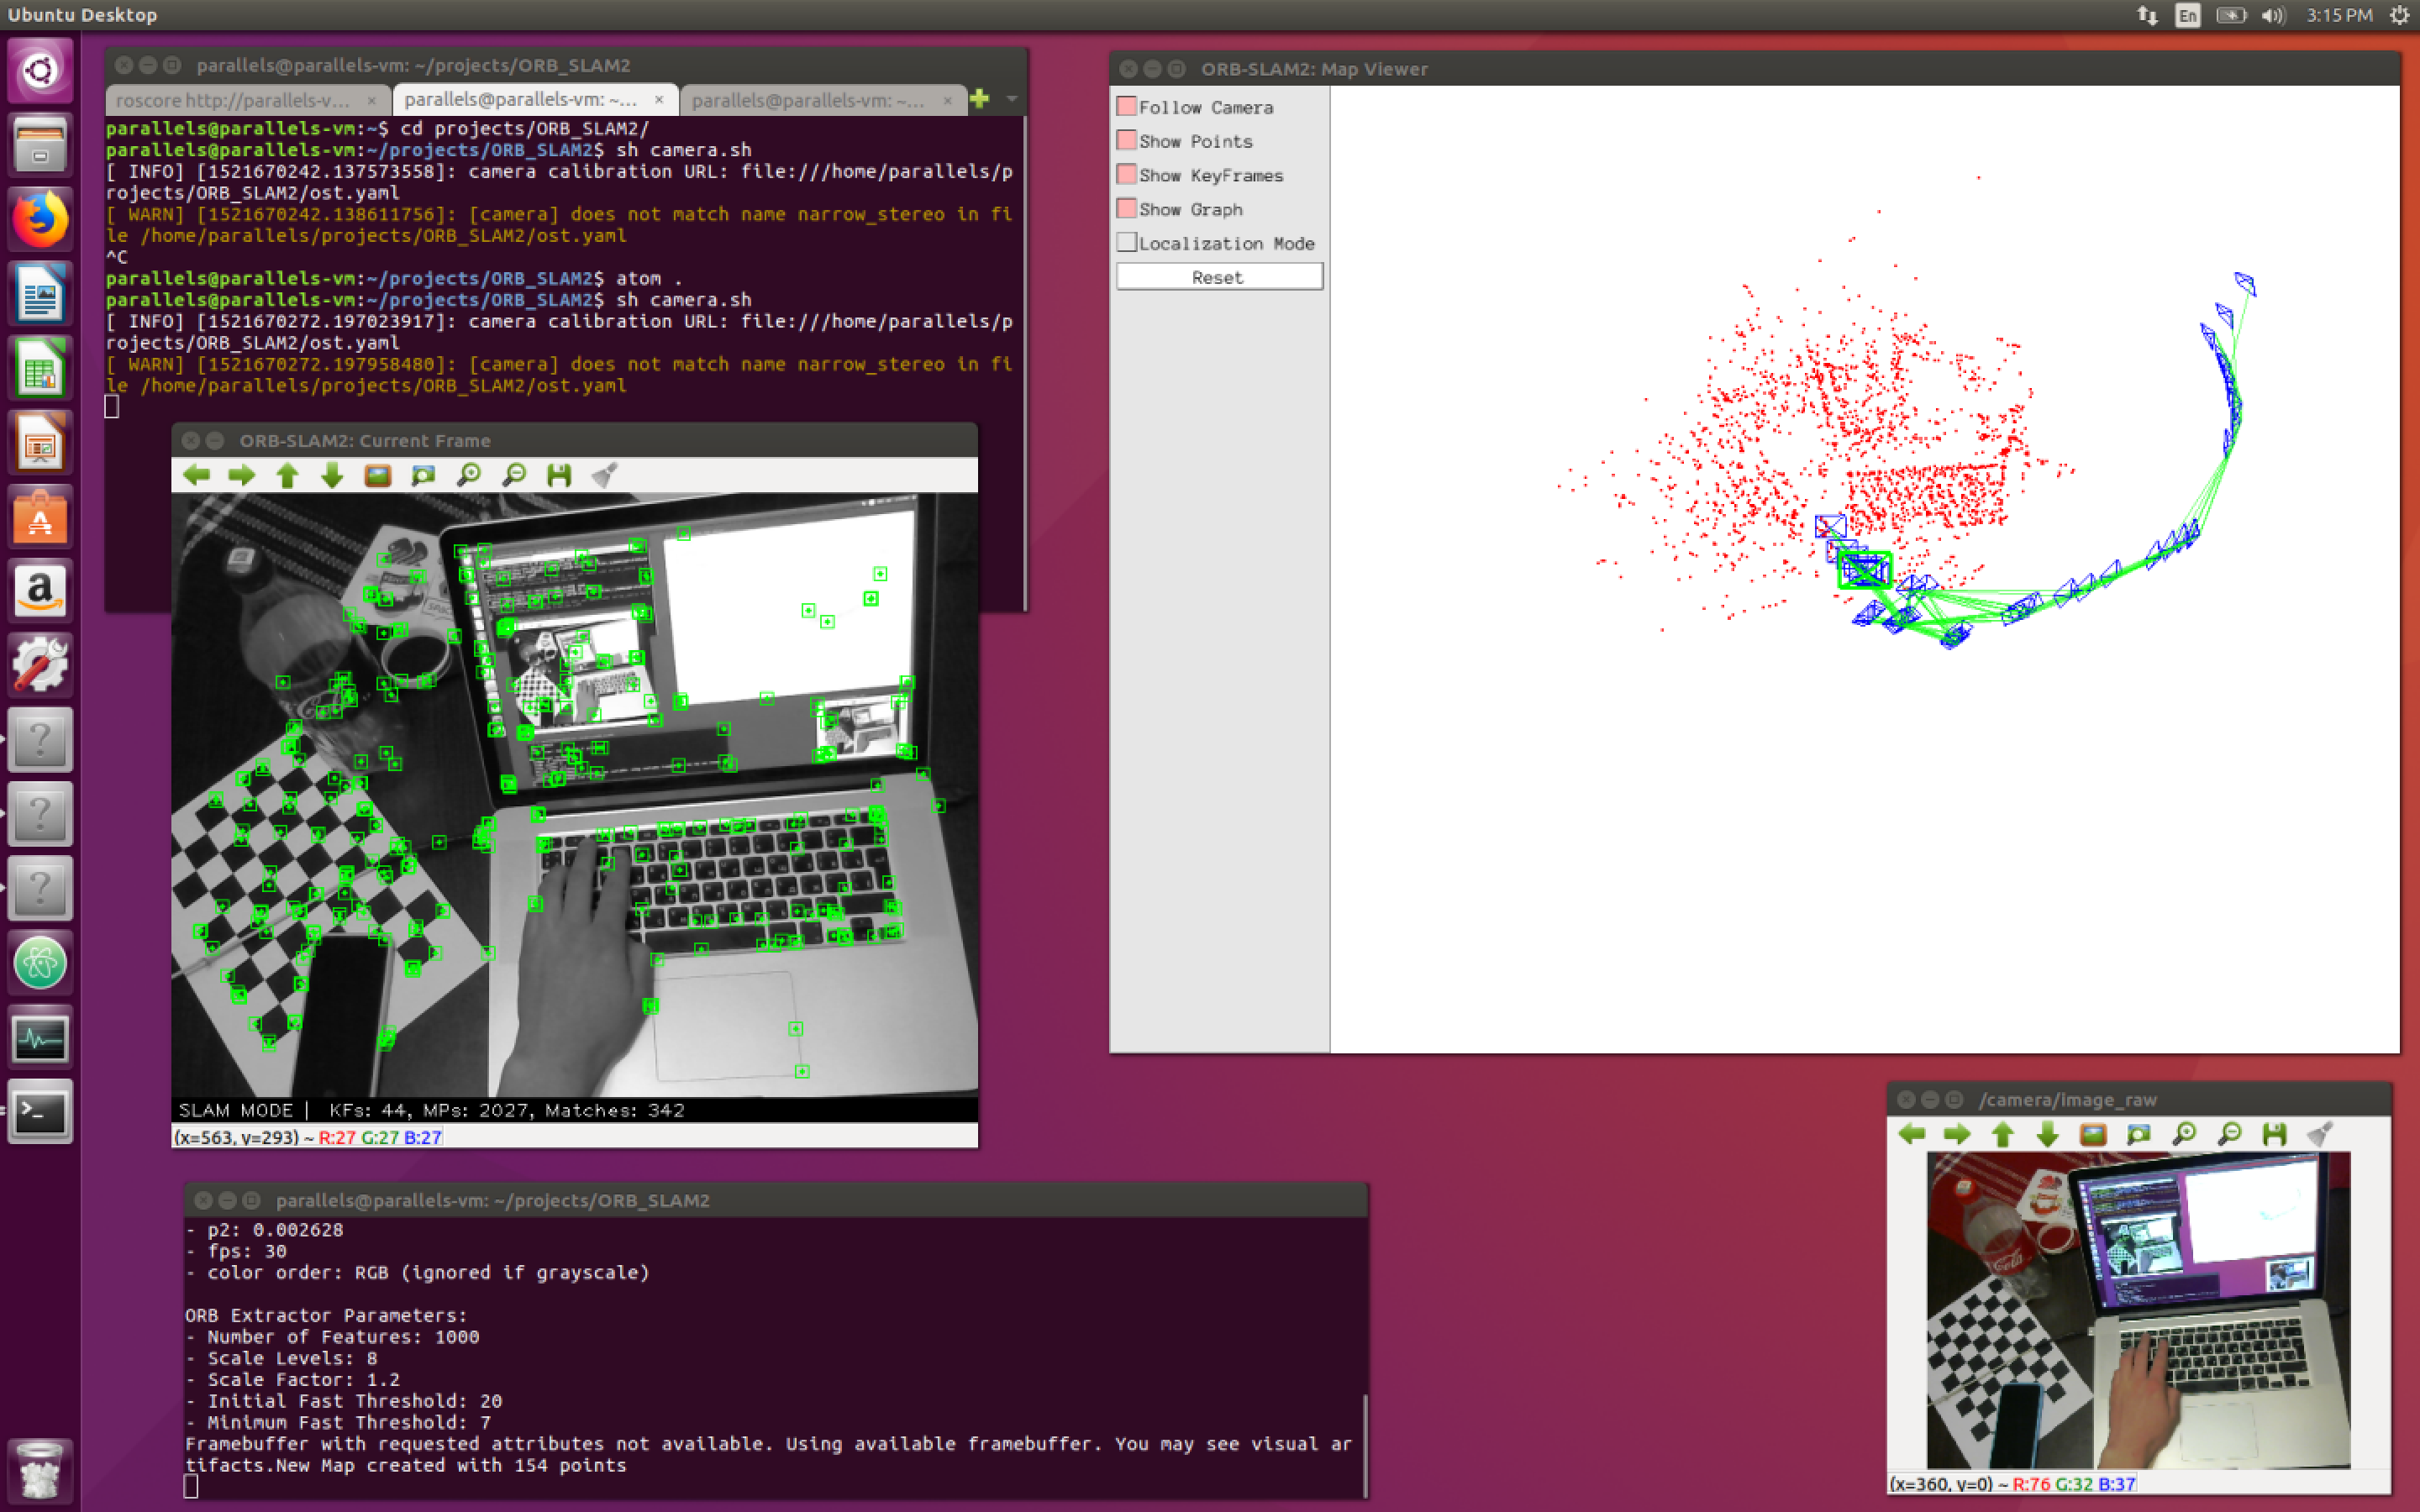
\includegraphics[width=1.0\textwidth]{images/ros-slam.png}
    \caption{Пример работы SLAM с веб-камерой}
    \label{fig:ros-slam}
\end{figure}